%------------------------------------------------
\section{Resultados}
%------------------------------------------------

%%%%%%%%%%%%%%%%%%%%%%%%%%%%%%%%%%%%%%%%%%%%%%%%%%%%%%%%%%%
%%%%%%%%%%%%%%%%%%%%%%%%%%%%%%%%%%%%%%%%%%%%%%%%%%%%%%%%%%%

\subsection{Projeto e implementação da estrutura mecânica}

\begin{frame}
\frametitle{Projeto e implementação da estrutura mecânica}
\begin{columns}

	\column{0.4\textwidth}
	\begin{itemize}
	\item \textit{Hardware} dividido em duas partes:
		\begin{itemize}
		\item Barra frontal de sensores
		\item Chassi (CrazyFrog)
		\end{itemize}
	\end{itemize}
	
	\column{0.6\textwidth}
	\begin{figure}[th]
	\centering
	\captionsetup{width=0.65\textwidth,font=footnotesize,textfont=bf}
	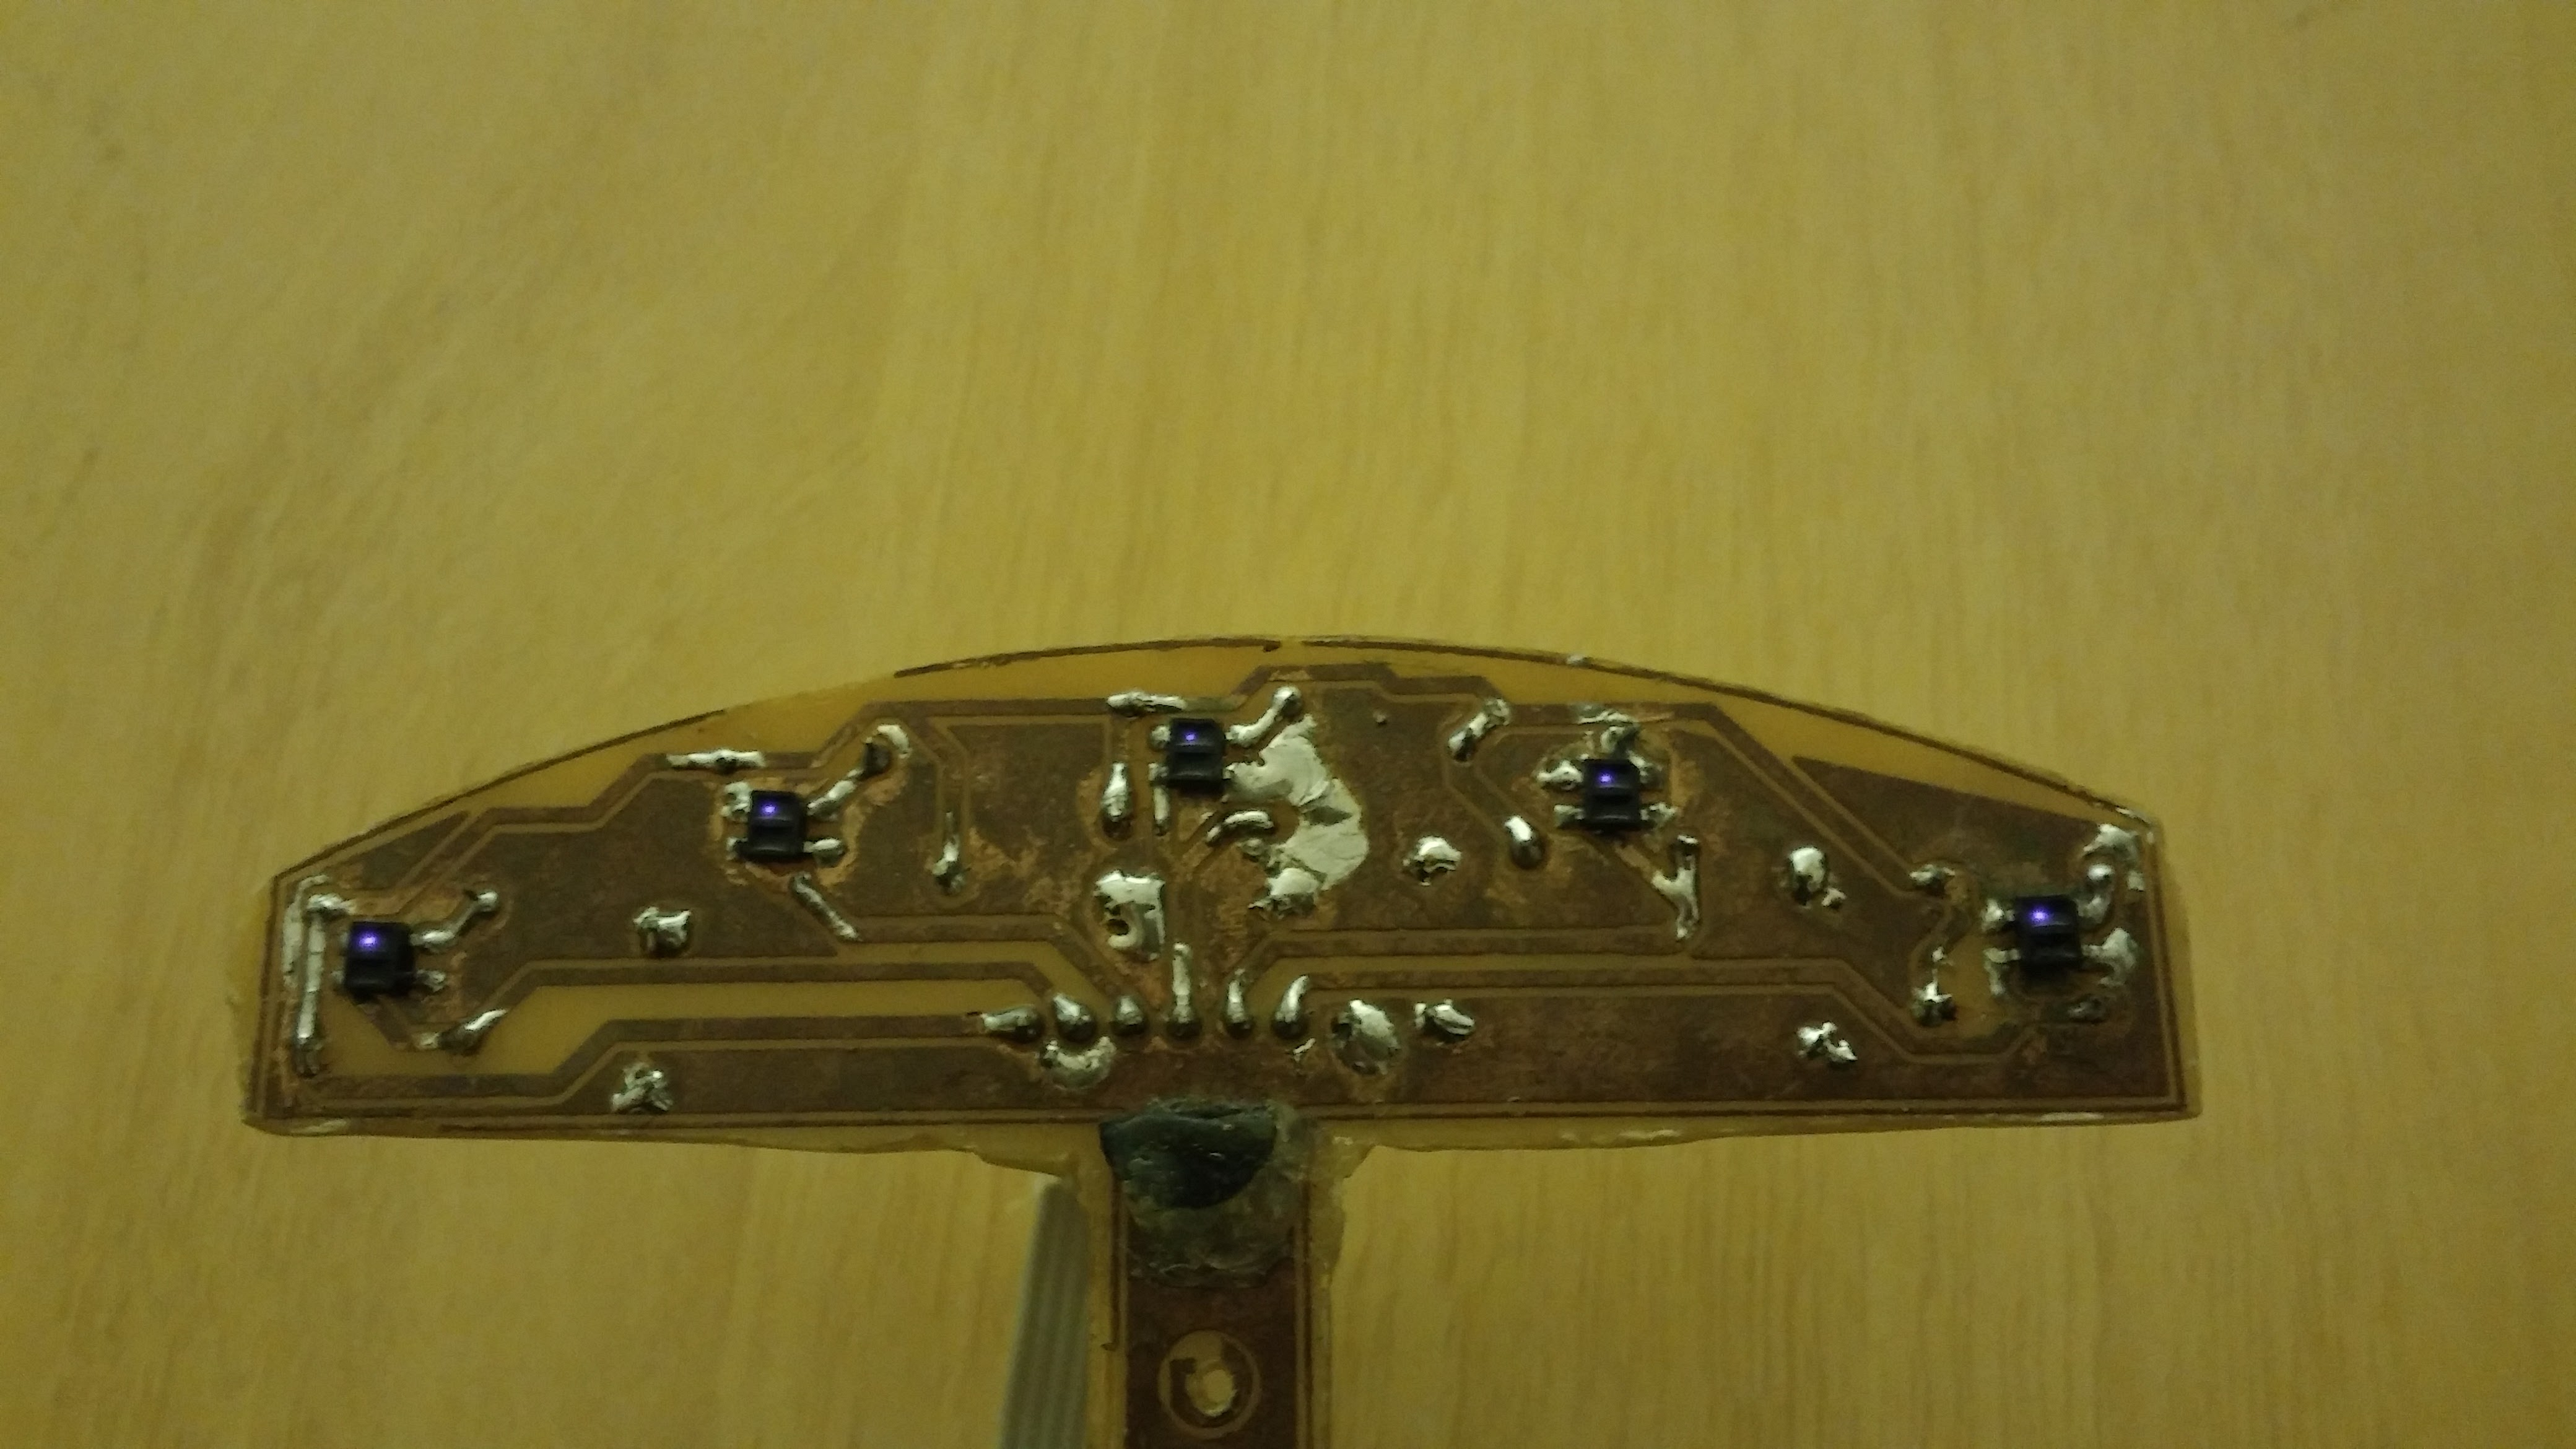
\includegraphics[width=0.65\textwidth,keepaspectratio]{Figuras/Barraluz.jpg}
	\caption{Barra frontal de sensores}
	\end{figure}

\end{columns}
\end{frame}


\begin{frame}
\frametitle{Projeto e implementação da estrutura mecânica}
\begin{figure}[h]
     \centering
     \captionsetup{width=0.8\textwidth,font=footnotesize,textfont=bf}
     \begin{subfigure}[b]{0.3\textwidth}
 	\centering
         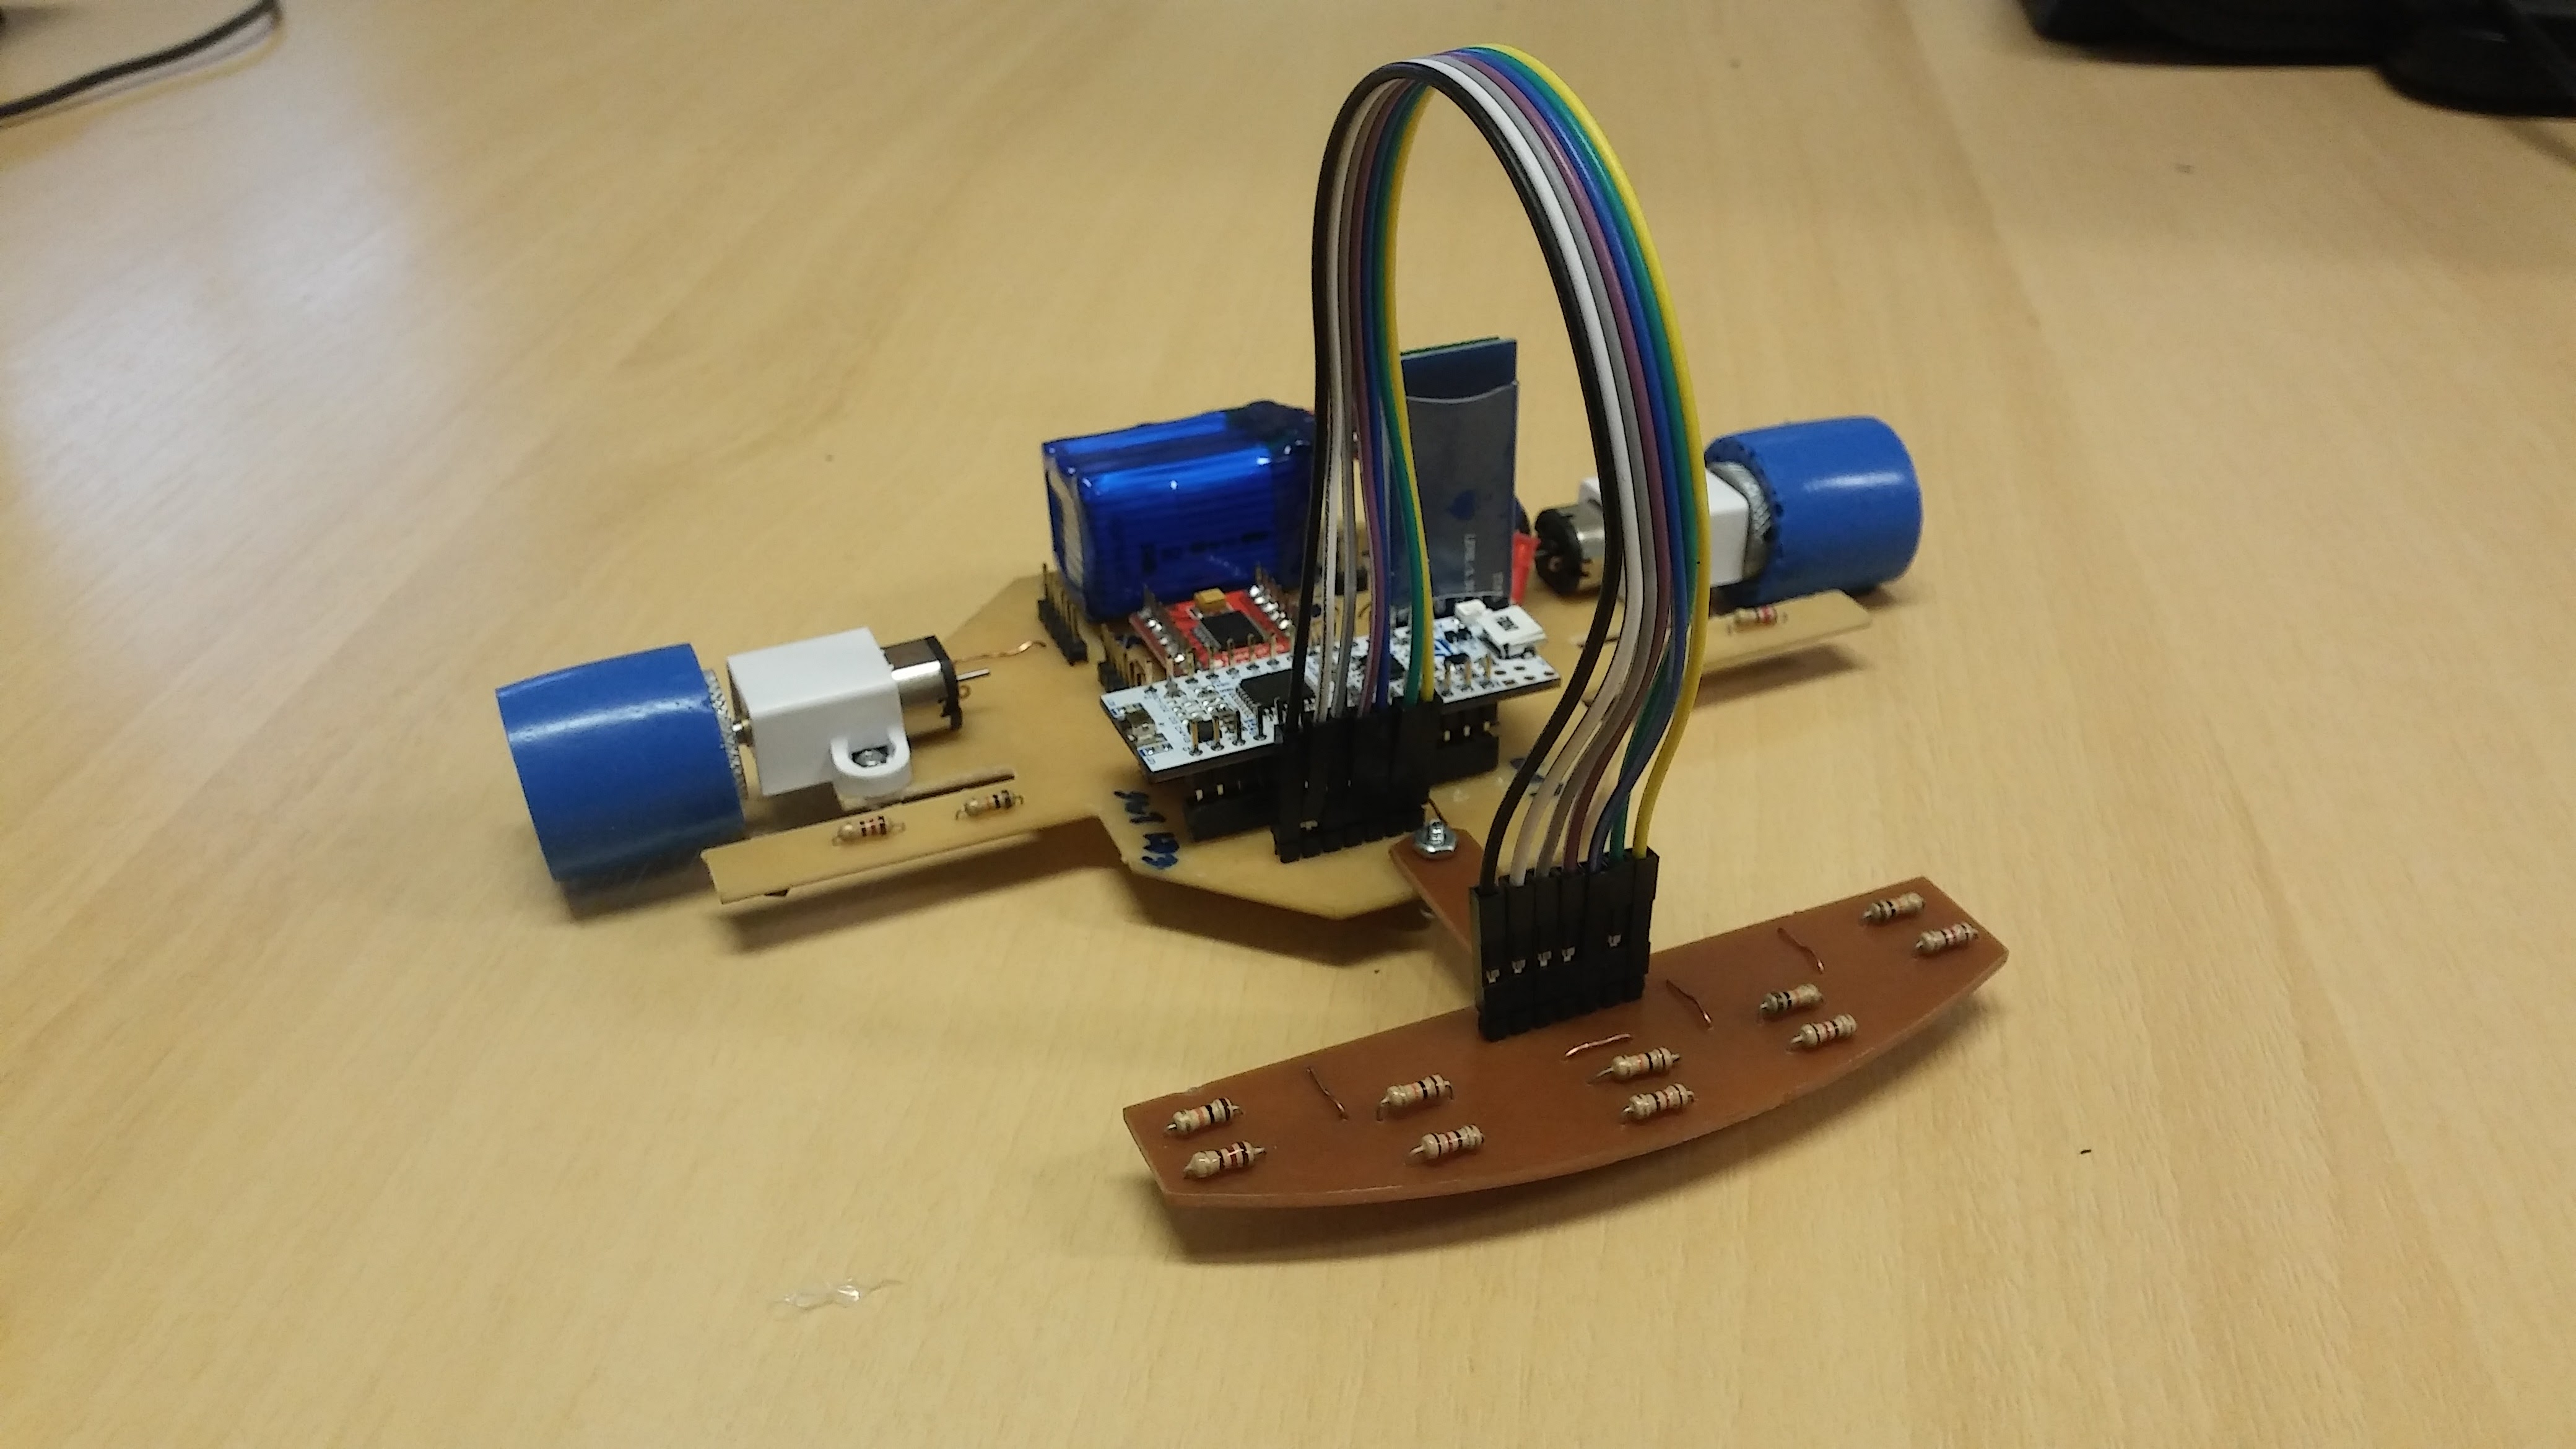
\includegraphics[width=\textwidth,height=\textheight,keepaspectratio]{figuras/crazy1.jpg}
         \caption{\centering}
     \end{subfigure}
     ~
     \pause
     \begin{subfigure}[b]{0.3\textwidth}
 	\centering
         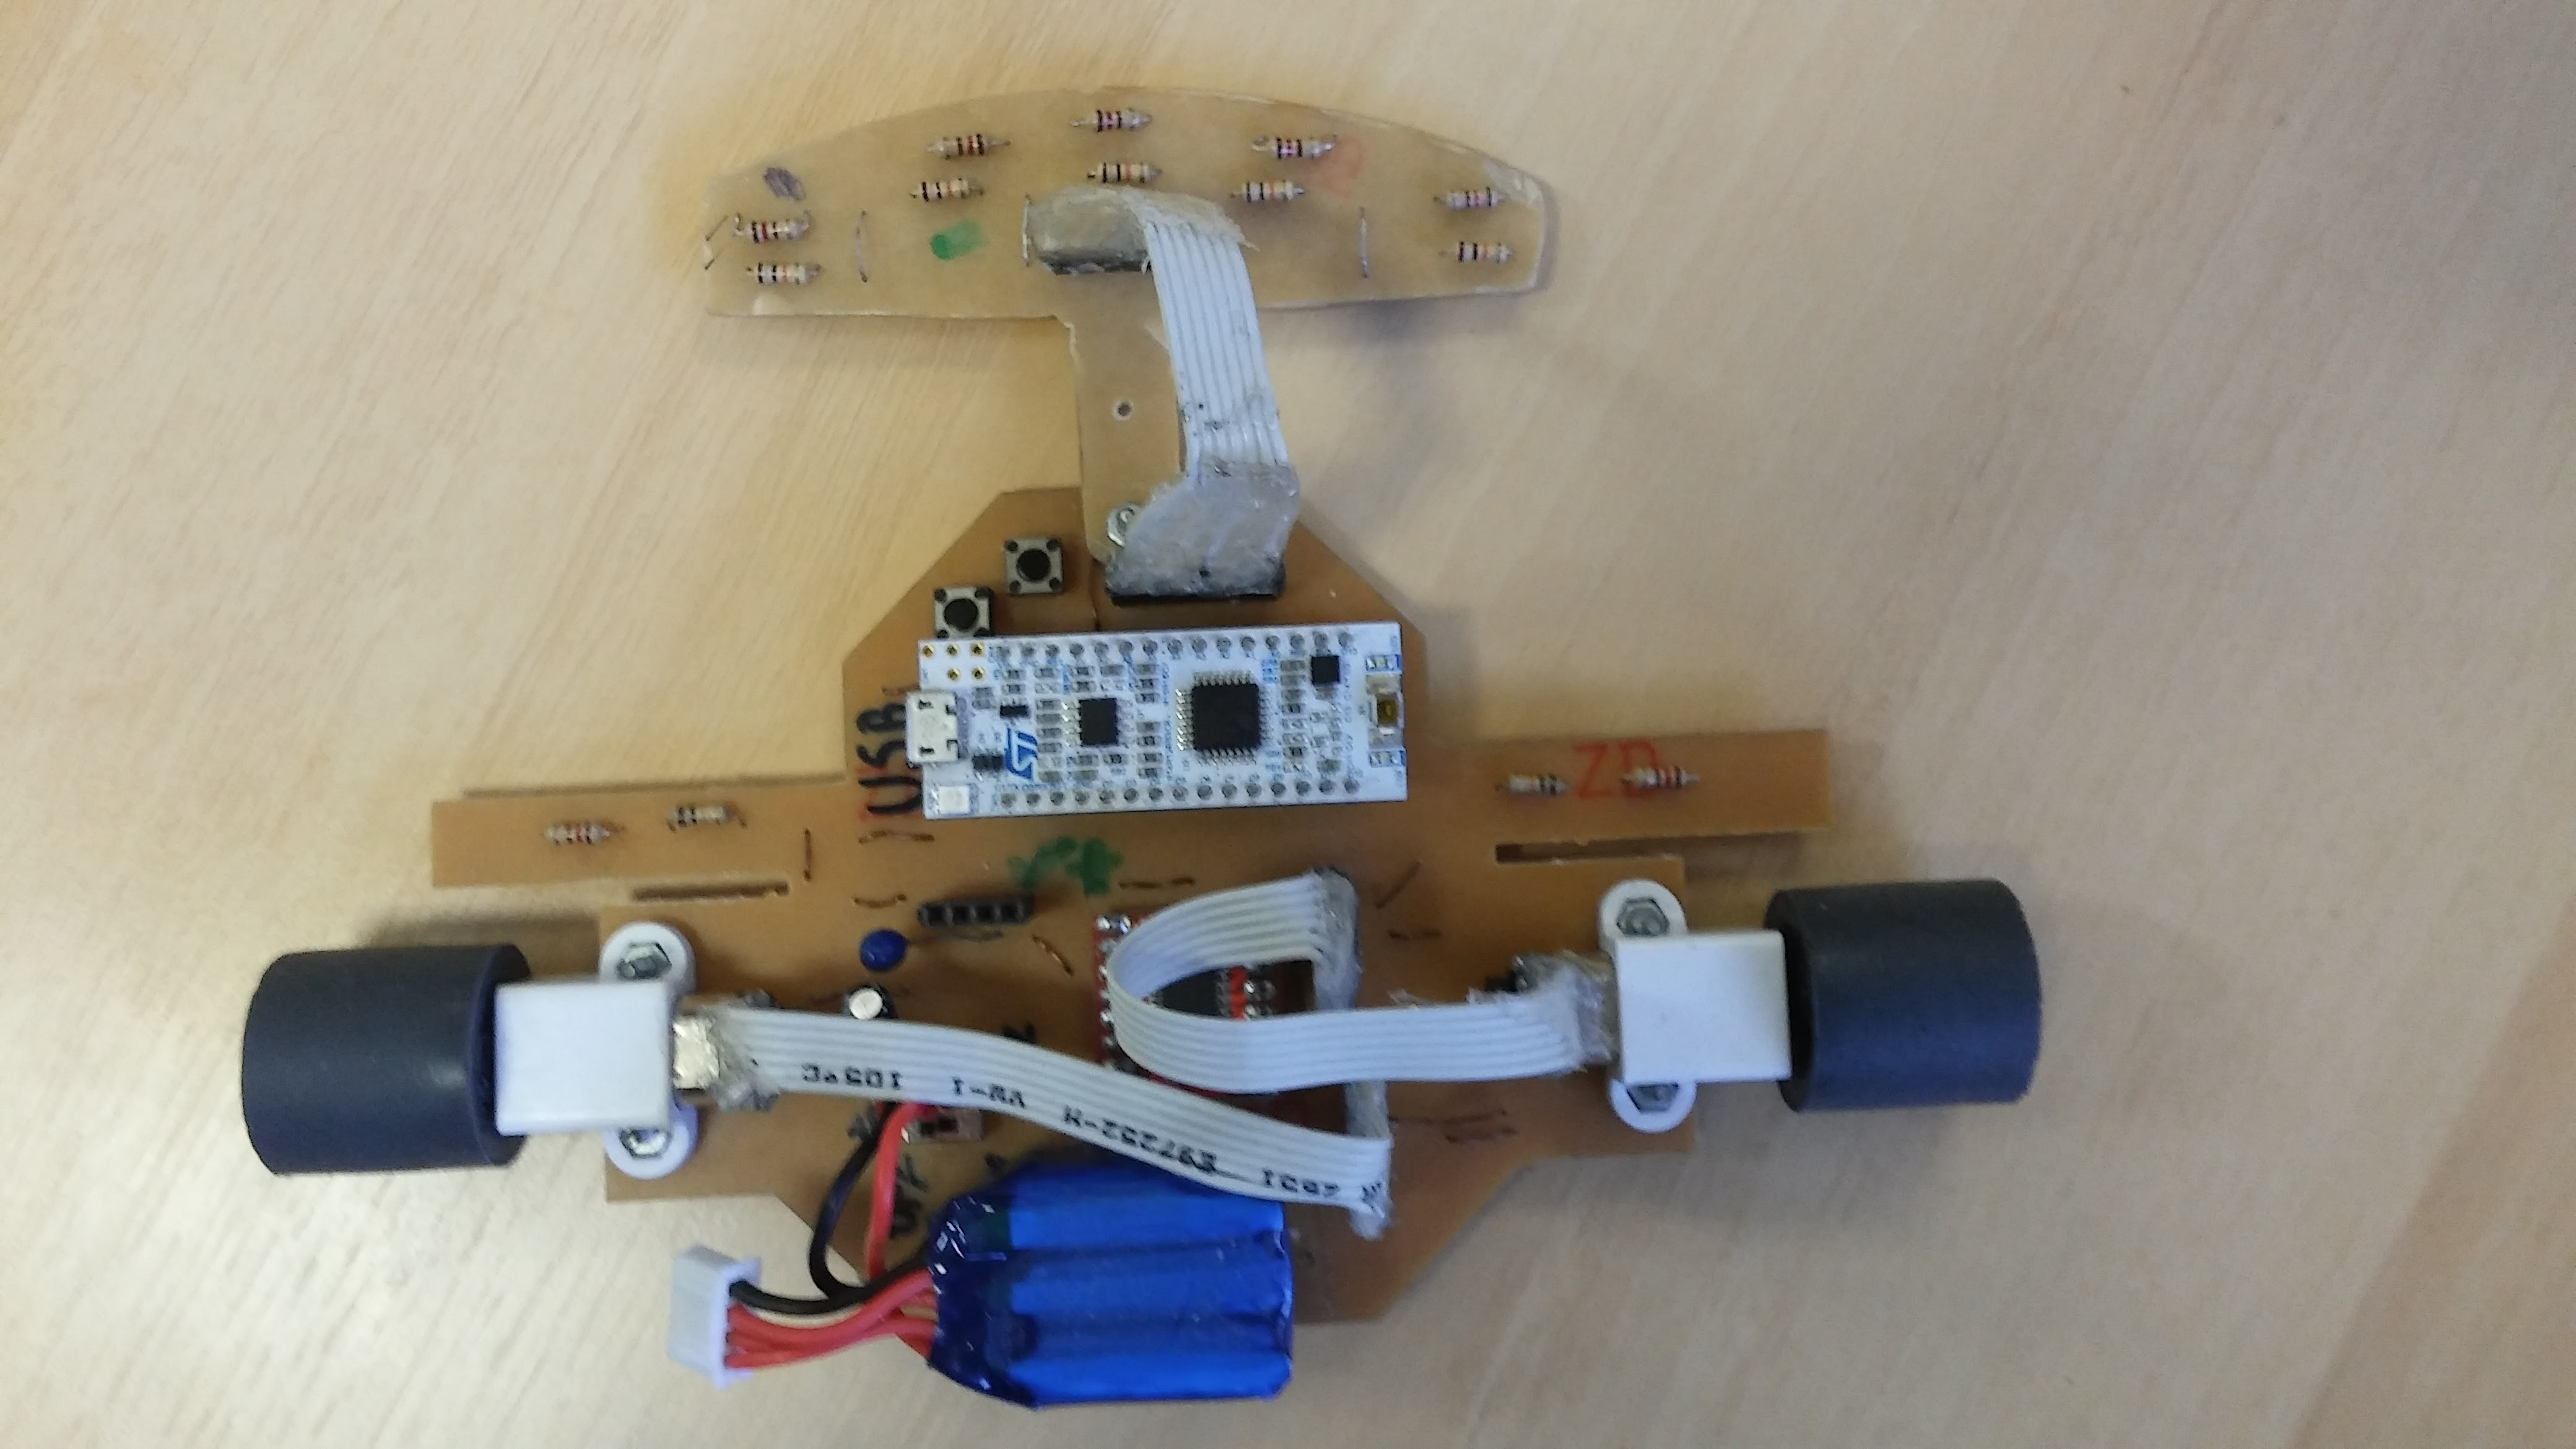
\includegraphics[width=\textwidth,height=5\textheight,keepaspectratio]{figuras/crazy2.jpg}
         \caption{\centering }
     \end{subfigure}
     ~
     \pause
     \begin{subfigure}[b]{0.3\textwidth}
 	\centering
         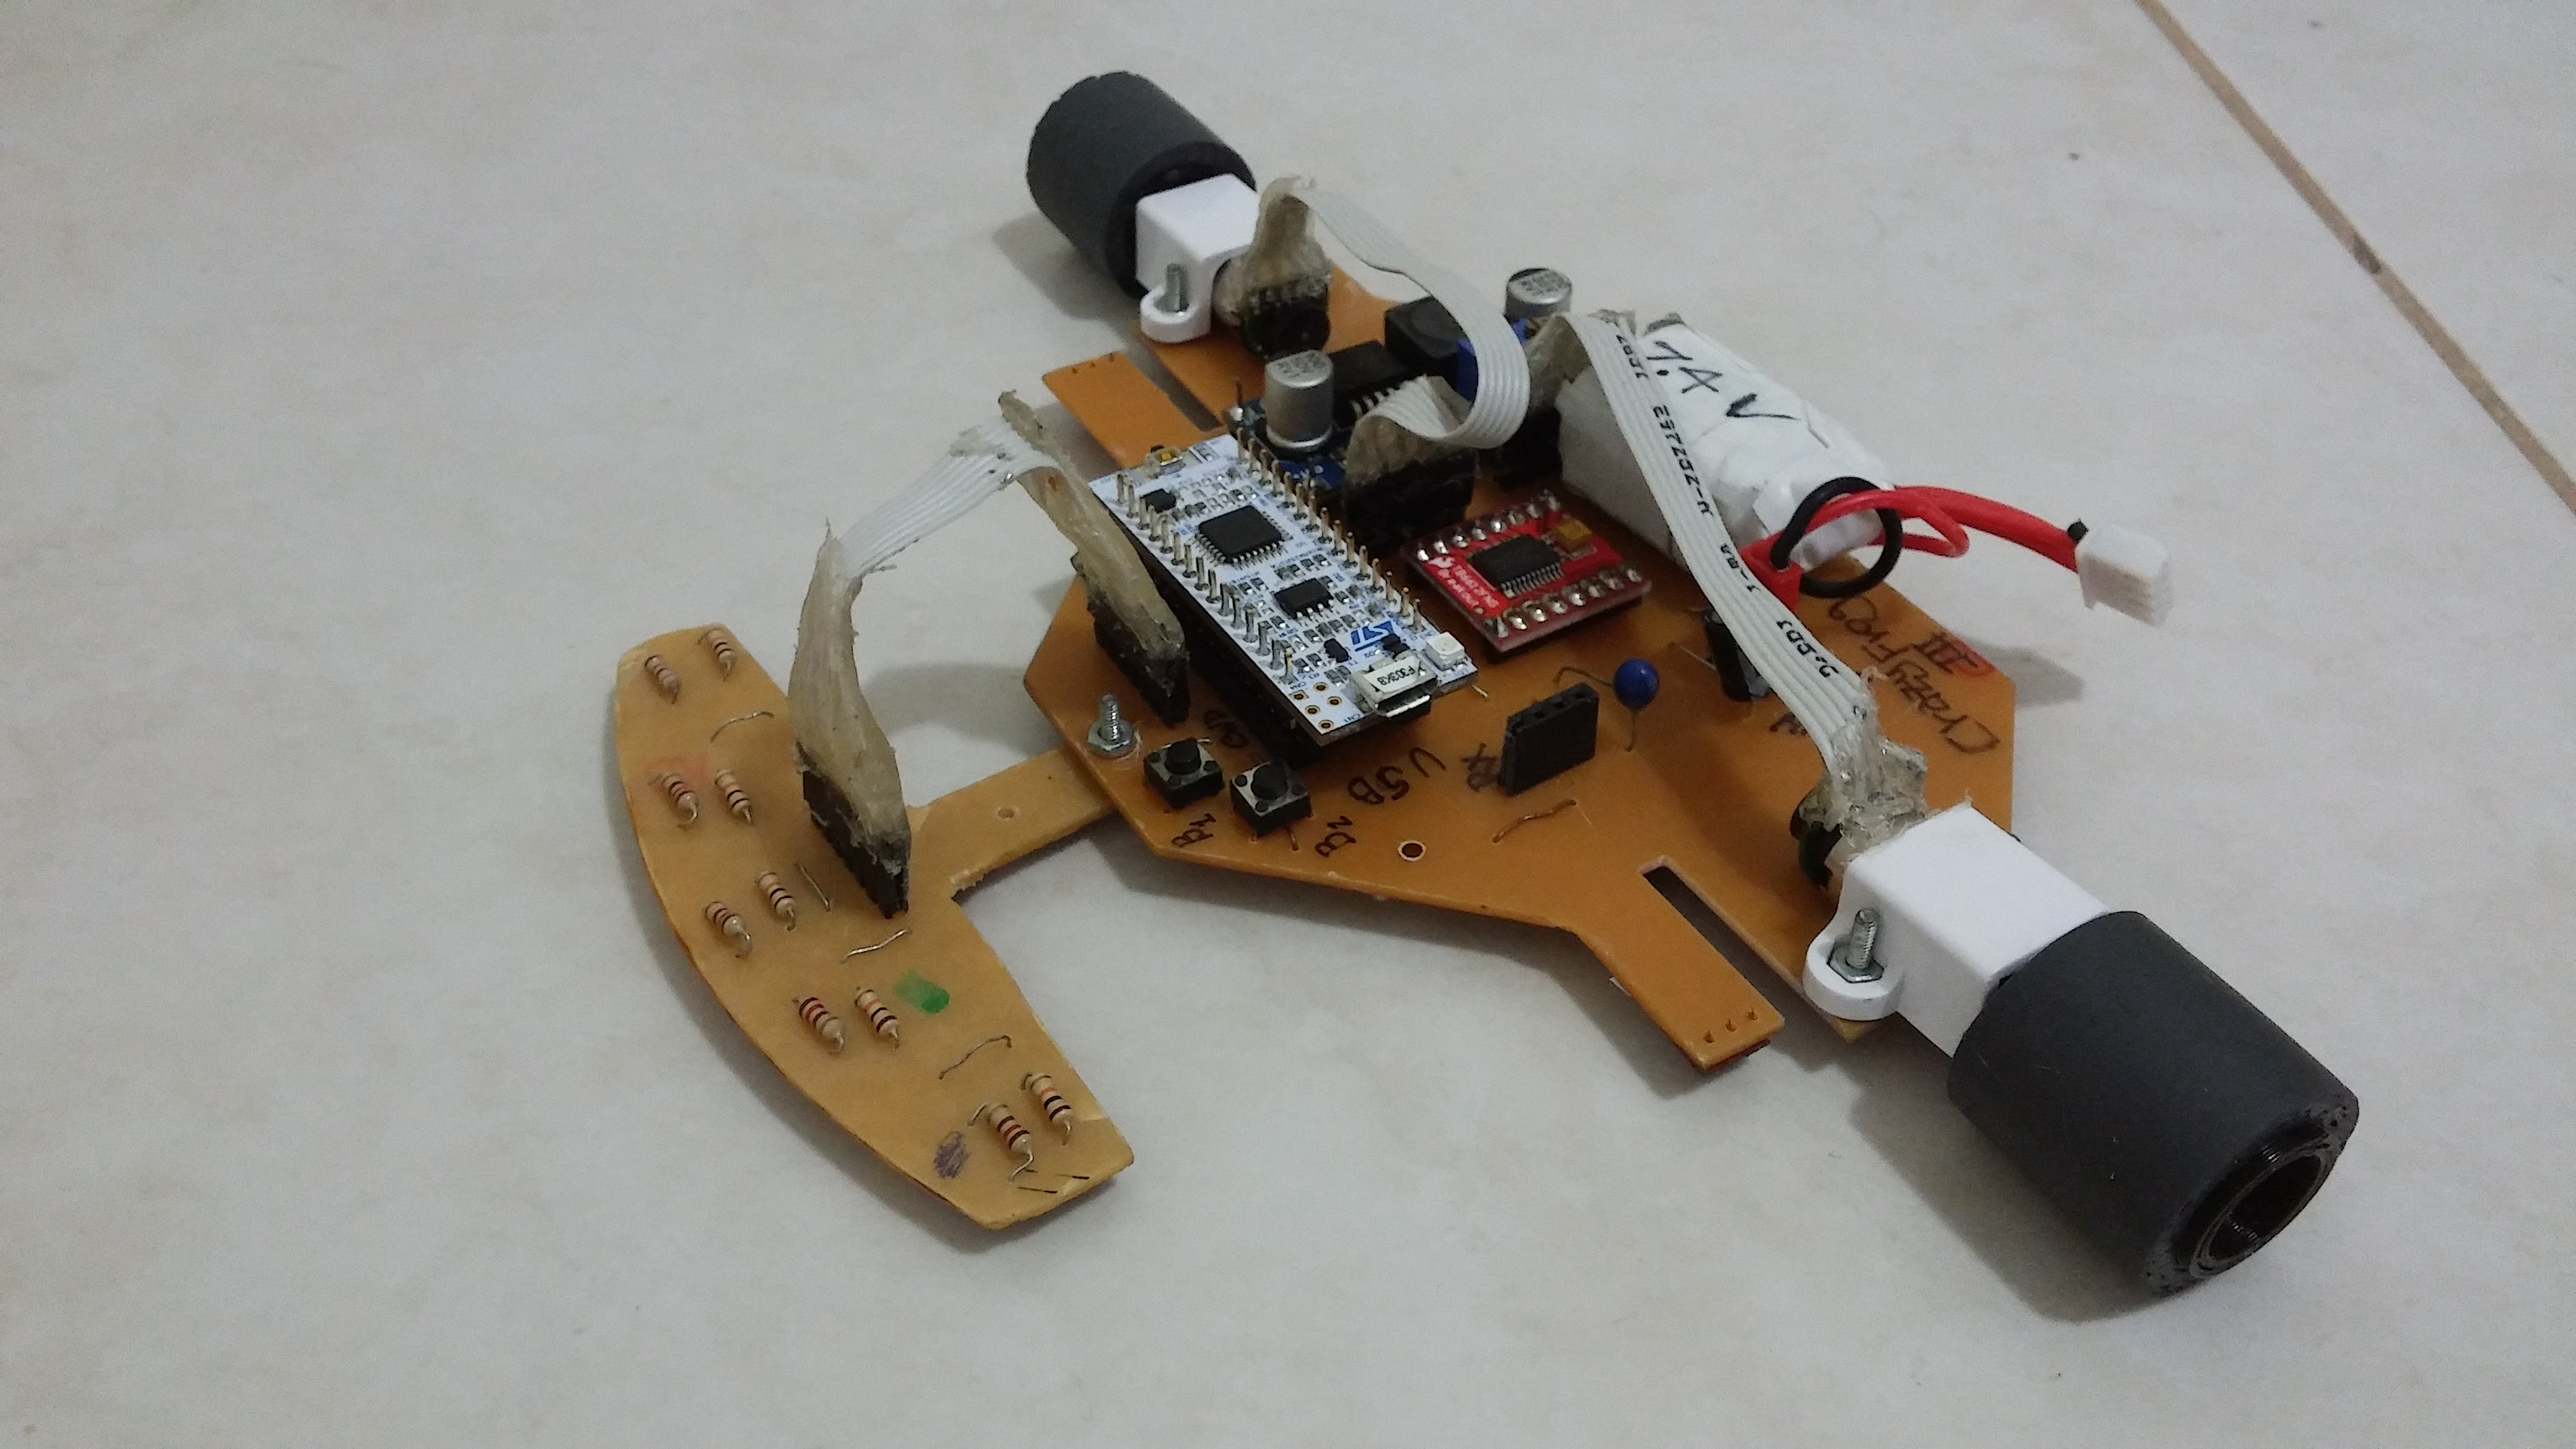
\includegraphics[width=\textwidth,height=5\textheight,keepaspectratio]{figuras/crazy3.jpg}
         \caption{\centering}
     \end{subfigure}
     \caption{Chassis desenvolvidos: (a) CrazyFrog1; (b) CrazyFrog2; (c) CrazyFrog3}

 \end{figure}
\end{frame}


%%%%%%%%%%%%%%%%%%%%%%%%%%%%%%%%%%%%%%%%%%%%%%%%%%%%%%%%%%%
%%%%%%%%%%%%%%%%%%%%%%%%%%%%%%%%%%%%%%%%%%%%%%%%%%%%%%%%%%%

\subsection{Participação em competições}

\begin{frame}
\frametitle{Participação em competições}
\begin{columns}

	\column{0.4\linewidth}
	\begin{itemize}
		\item Participação na FACE e WinterChallenge
		\item Competições disputadas com o CrazyFrog2
		\item Problema com os sensores
		\item Curva do 'S'
	\end{itemize}		
	
	
	\column{0.6\linewidth}
	\begin{figure}[th]
	\centering
	\captionsetup{width=\textwidth,font=footnotesize,textfont=bf}
	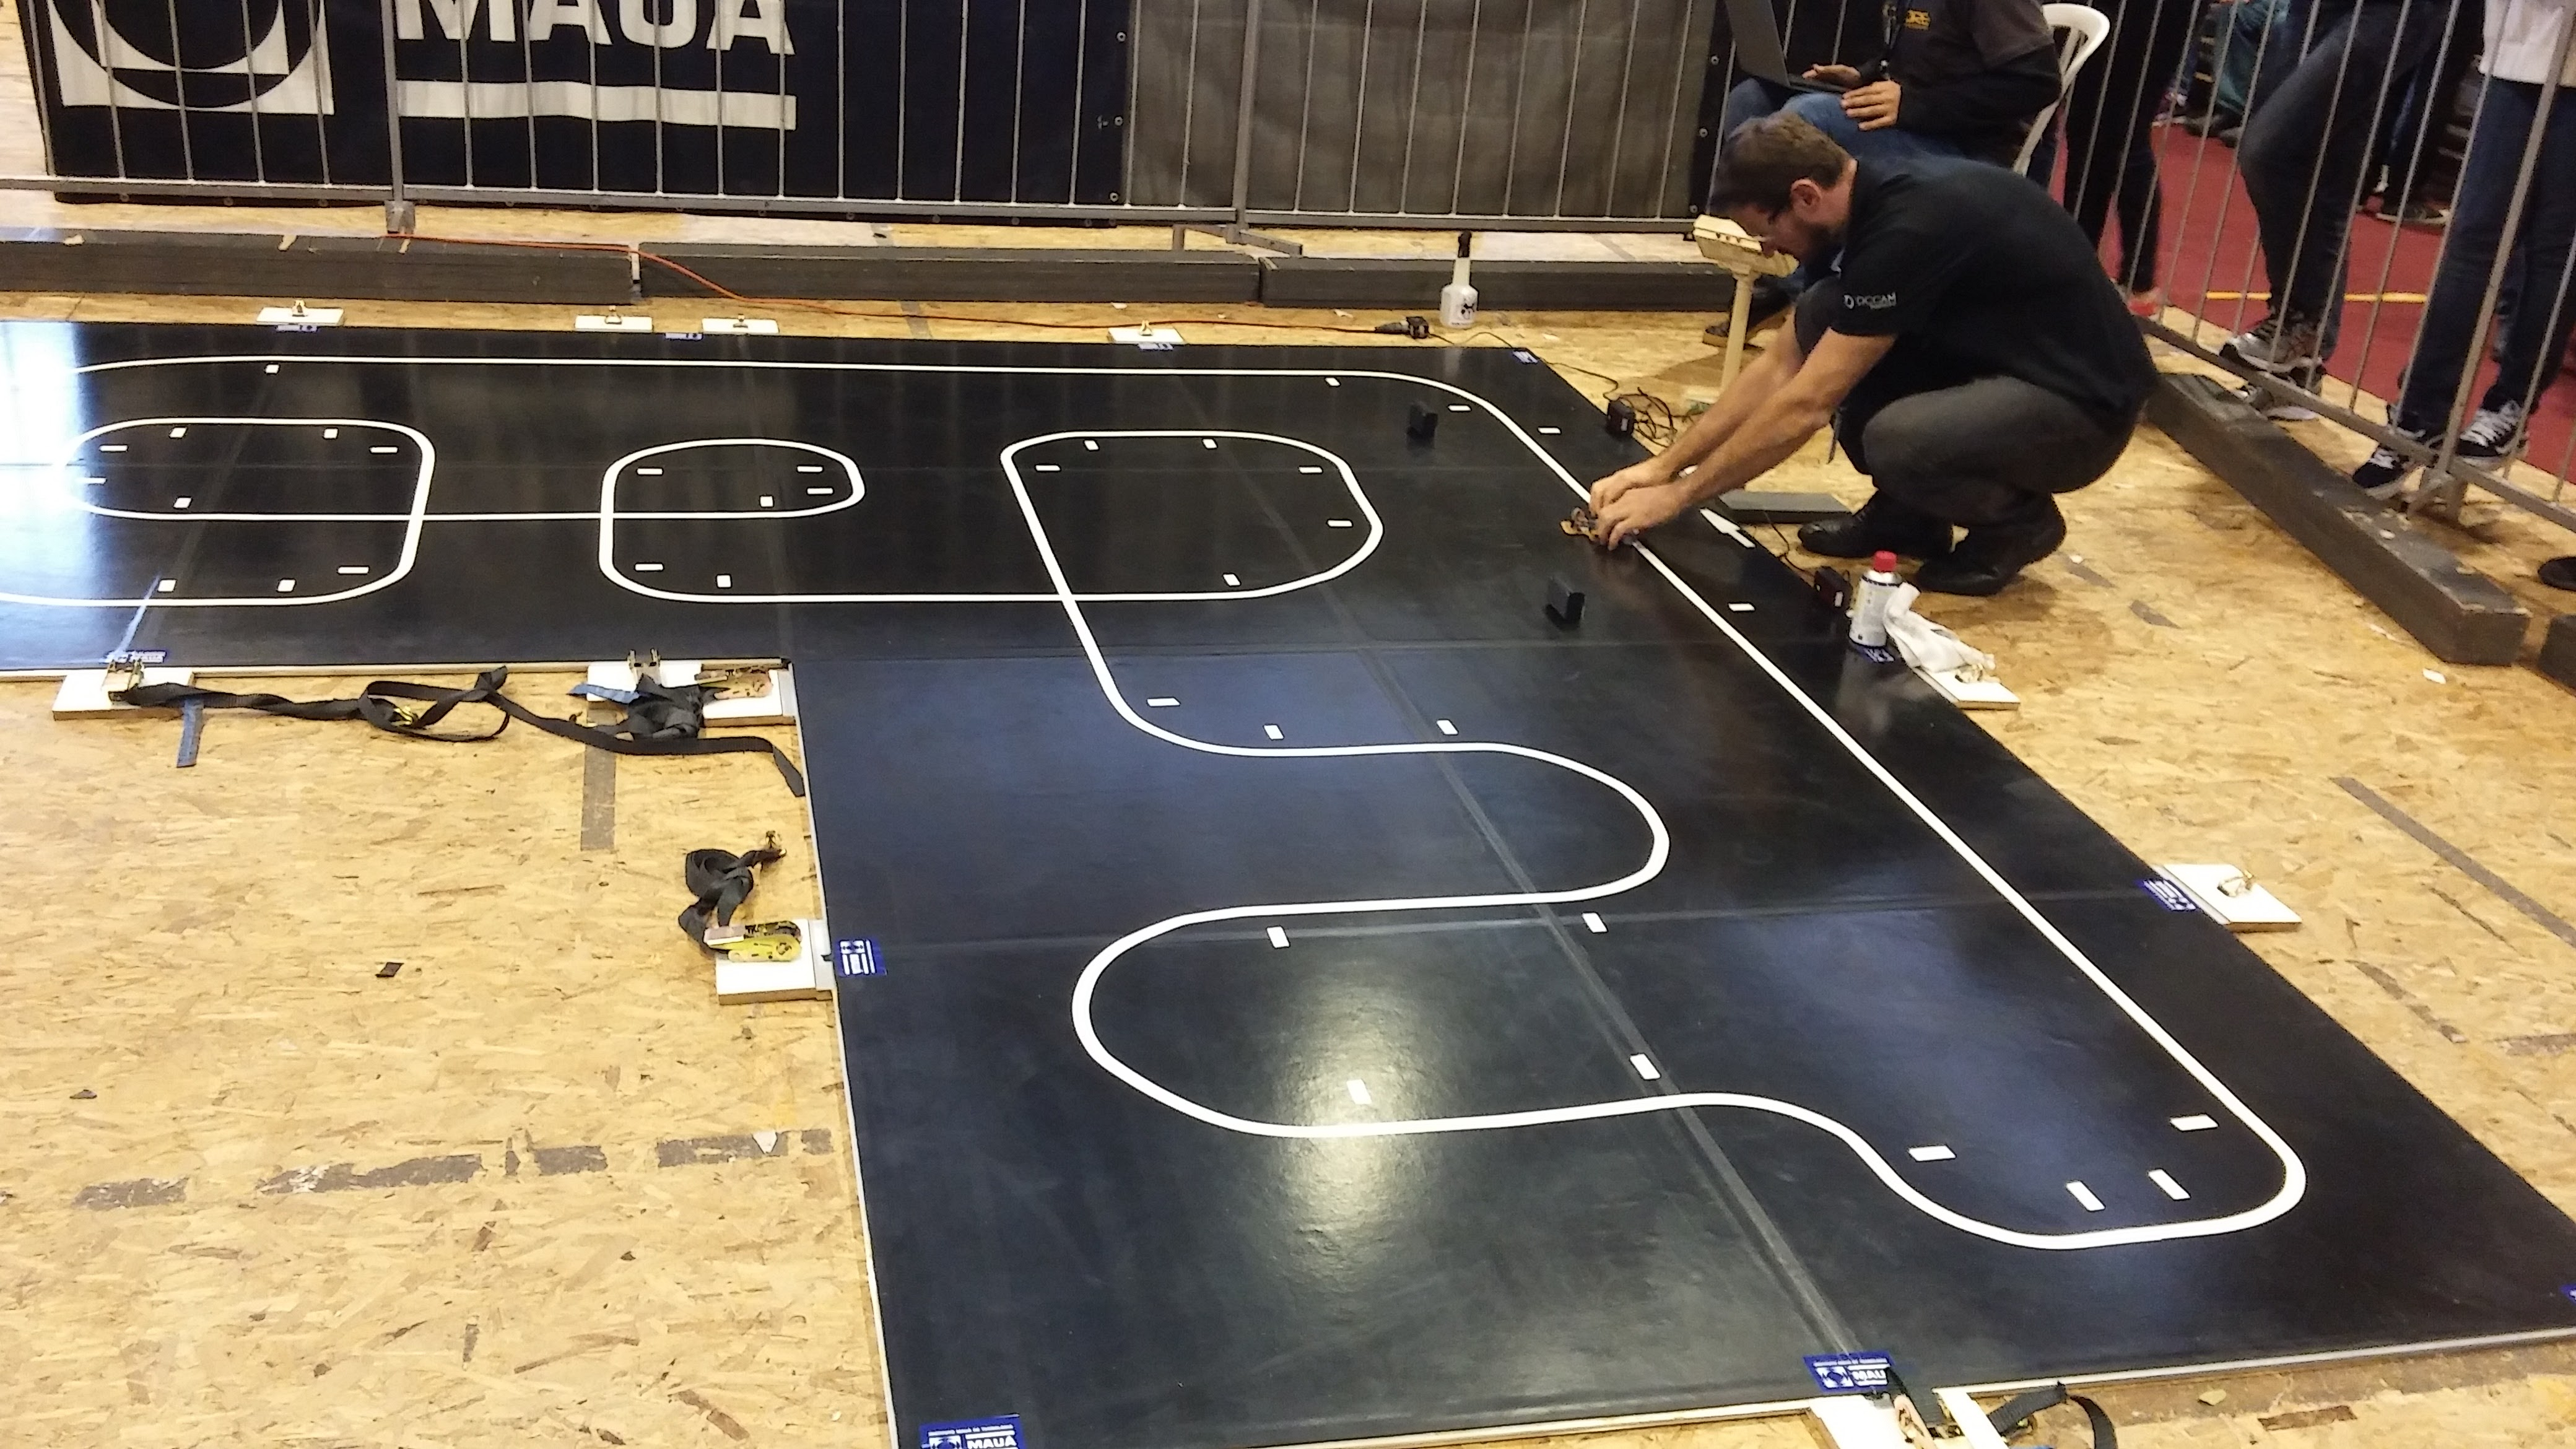
\includegraphics[width=\textwidth,keepaspectratio]{Figuras/winter.jpg}
	\caption{Pista do seguidor de linha Pro na WinterChallenge2017}
	\end{figure}
	
\end{columns}
\end{frame}

%%%%%%%%%%%%%%%%%%%%%%%%%%%%%%%%%%%%%%%%%%%%%%%%%%%%%%%%%%%
%%%%%%%%%%%%%%%%%%%%%%%%%%%%%%%%%%%%%%%%%%%%%%%%%%%%%%%%%%%

\subsection{Teste dos sensores de refletância}

\begin{frame}
\frametitle{Teste dos sensores de refletância}
\begin{columns}

	\column{0.4\linewidth}
	\begin{itemize}
		\item Sensores testados
		\begin{itemize}
			\item QTR-1A, da Pololu;
			\item QRE1113, da China;
			\item QRE1113, da Arrow;
			\item QRD1114.
		\end{itemize}
		\item Procedimento para a aquisição
	\end{itemize}		
	
	
	\column{0.6\linewidth}
	\begin{figure}[th]
	\centering
	\captionsetup{width=\textwidth,font=footnotesize,textfont=bf}
	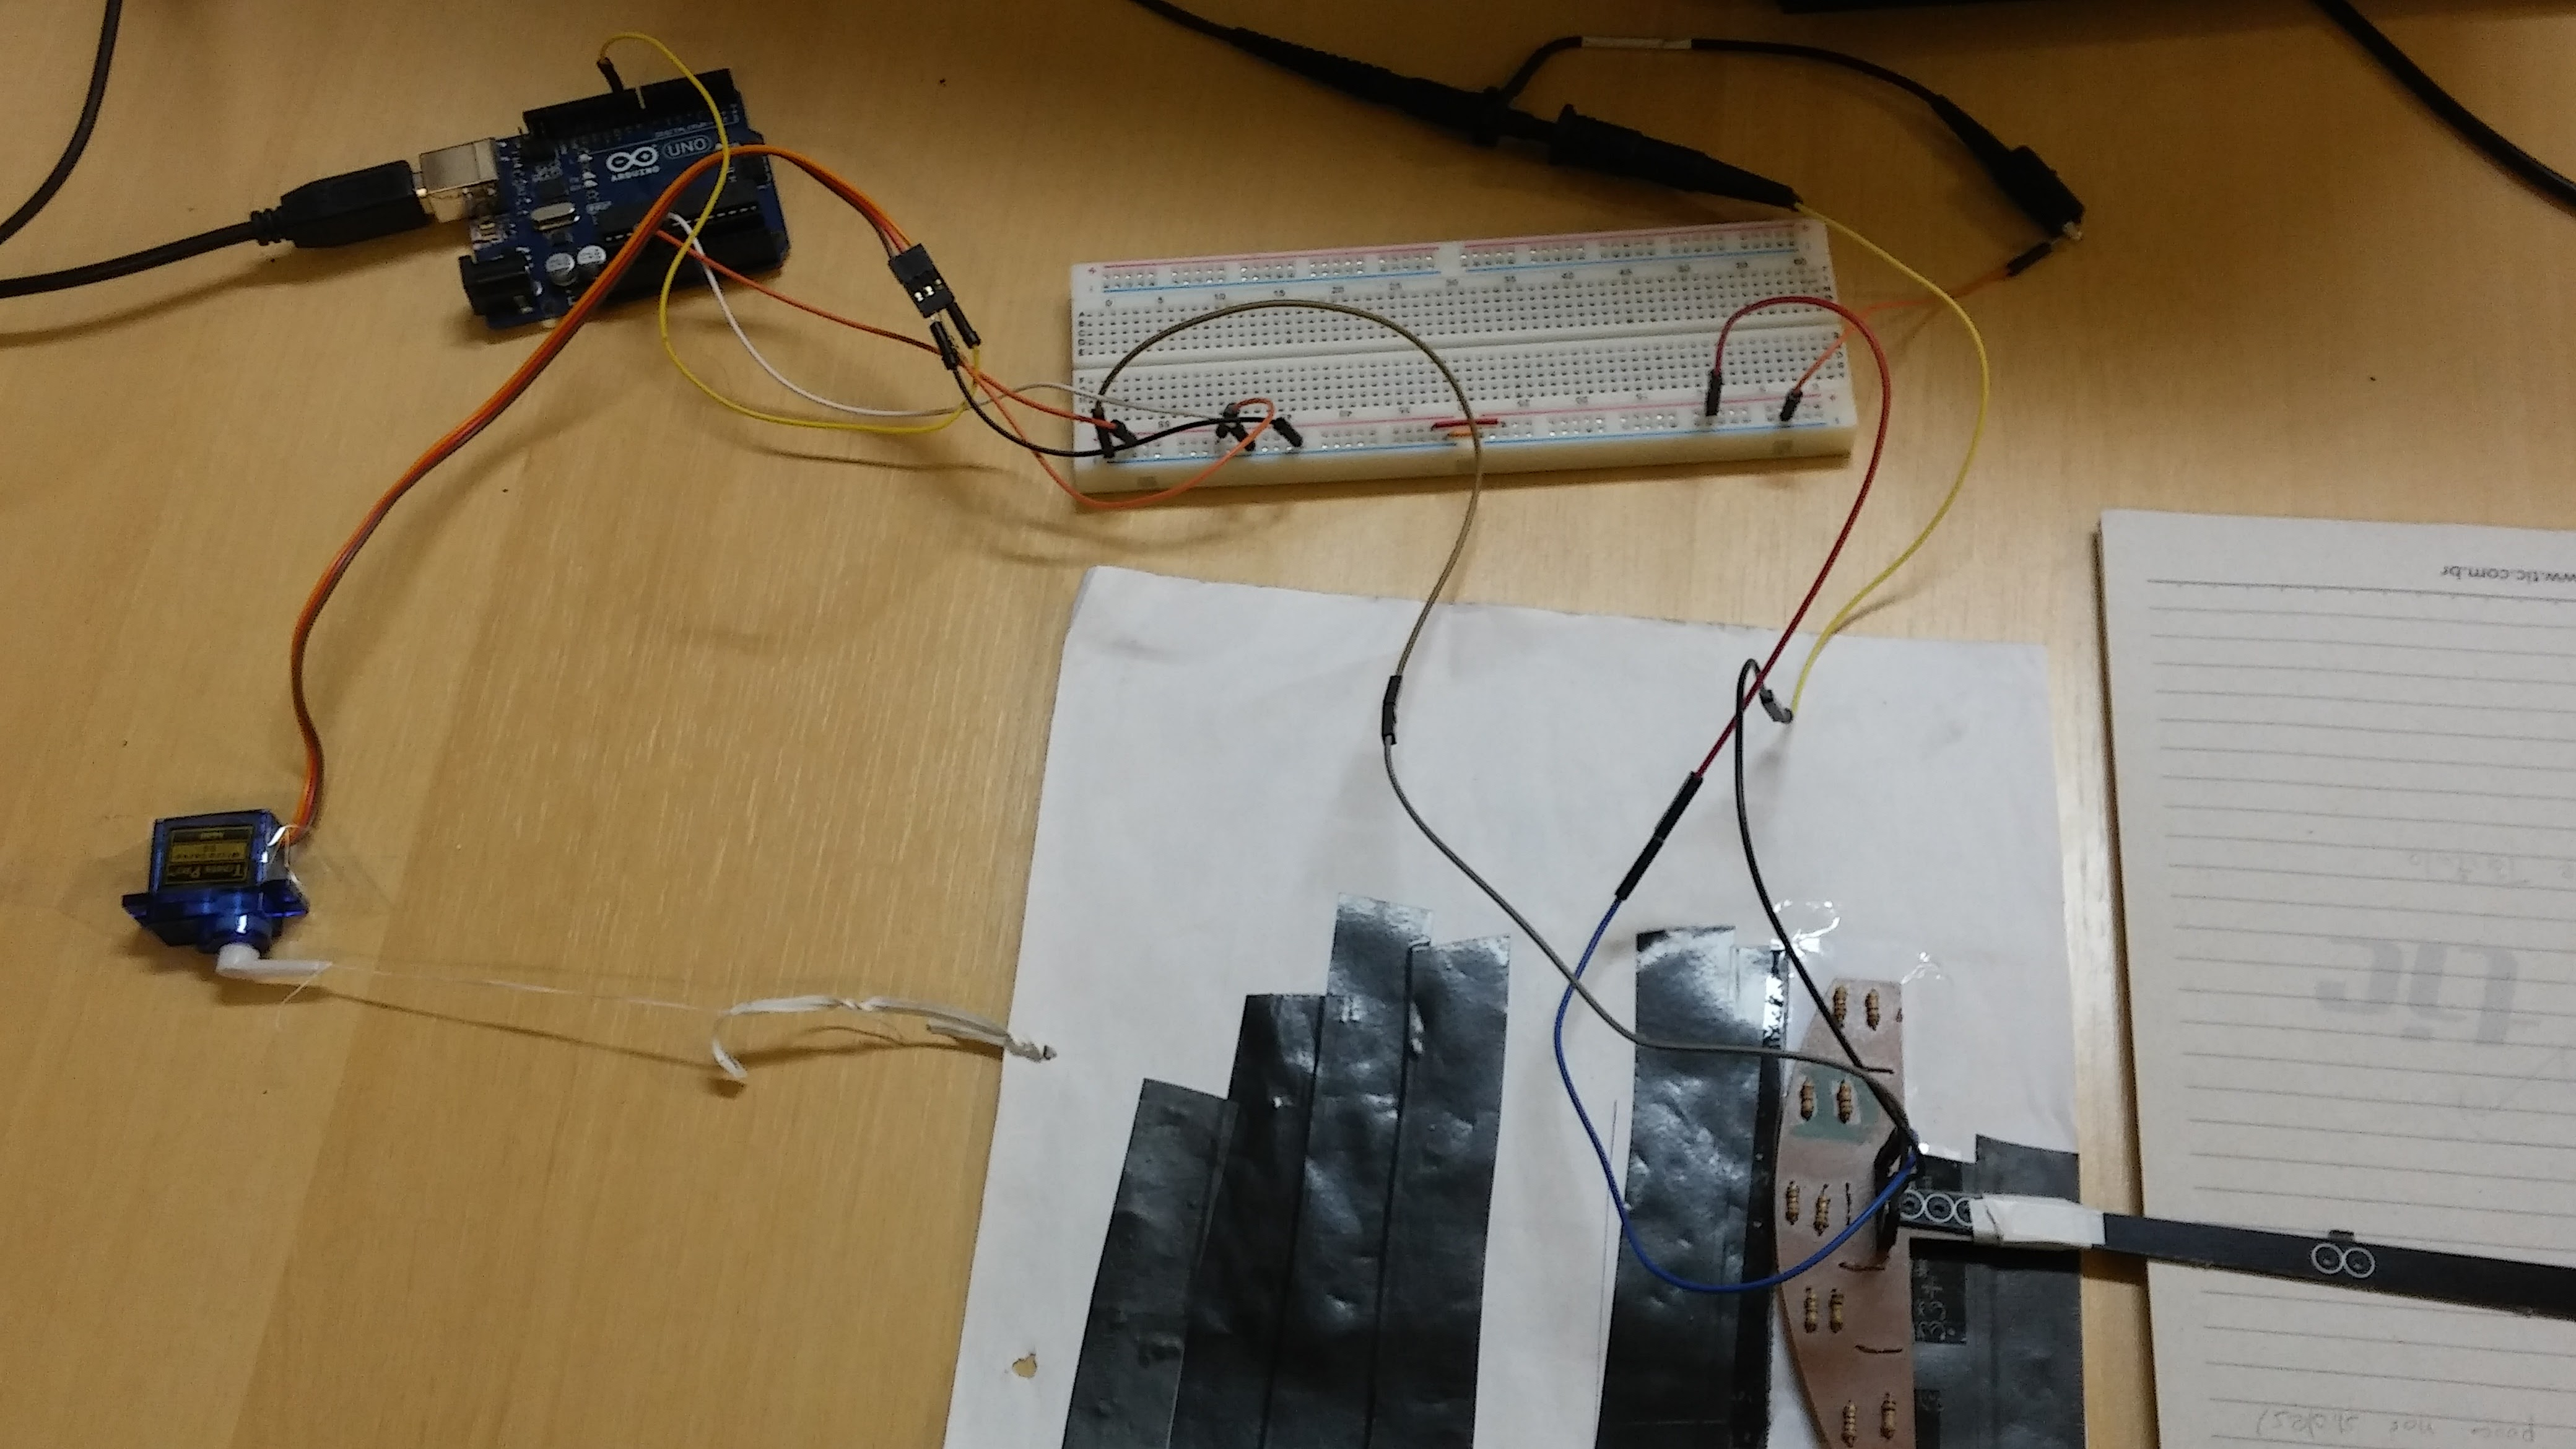
\includegraphics[width=\textwidth,keepaspectratio]{Figuras/mecanismo.jpg}
	\caption{Mecanismo de aquisição do tempo de resposta dos sensores}
	\end{figure}
	
\end{columns}
\end{frame}

\begin{frame}
\frametitle{Teste dos sensores de refletância}
 \begin{figure}[h]
     \centering
     \captionsetup{width=0.8\textwidth,font=footnotesize,textfont=bf}
     \begin{subfigure}[b]{0.3\textwidth}
 	\centering
         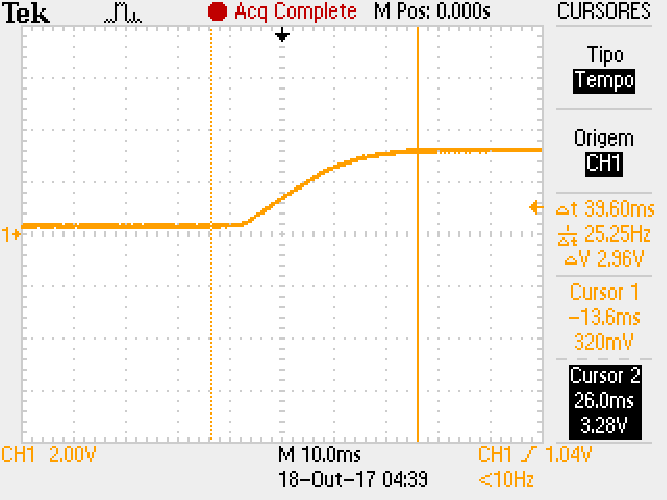
\includegraphics[width=\textwidth,height=\textheight,keepaspectratio]{figuras/TesteNew1mm.pdf}
         \caption{\centering \label{fig:TesteNew1mm}}
     \end{subfigure}
     ~
     \begin{subfigure}[b]{0.3\textwidth}
 	\centering
         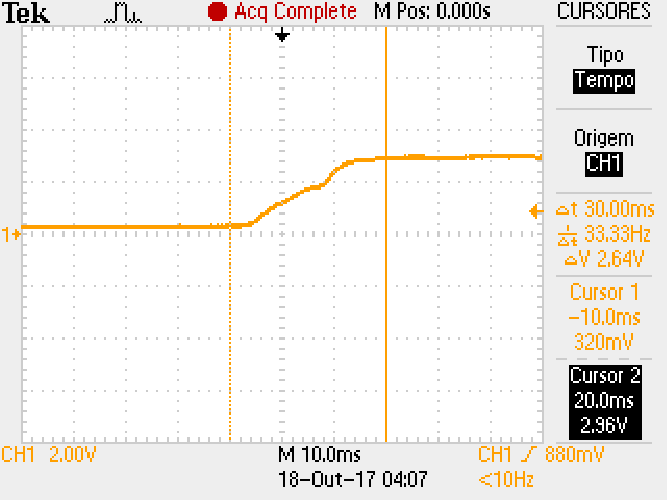
\includegraphics[width=\textwidth,height=5\textheight,keepaspectratio]{figuras/TesteOld1mm.pdf}
         \caption{\centering \label{fig:TesteOld1mm}}
     \end{subfigure}
     
     \captionsetup{width=\textwidth,font=footnotesize,textfont=bf}
     \begin{subfigure}[b]{0.3\textwidth}
 	\centering
         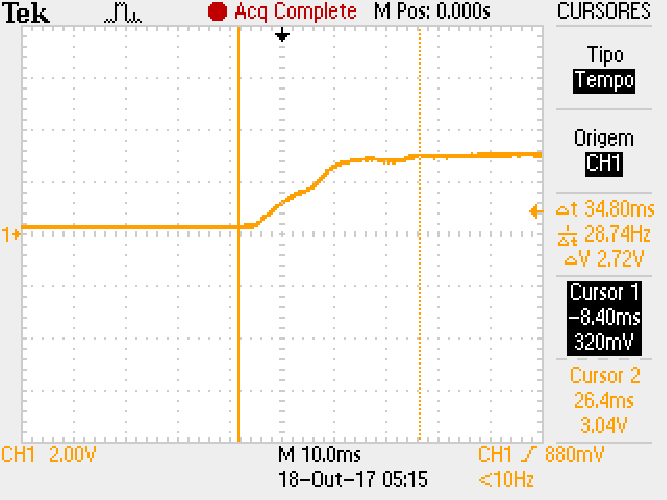
\includegraphics[width=\textwidth,height=\textheight,keepaspectratio]{figuras/TestePaulo1mm.pdf}
         \caption{\centering \label{fig:TestePaulo1mm}}
     \end{subfigure}
     ~ 
     \begin{subfigure}[b]{0.3\textwidth}
 	\centering
         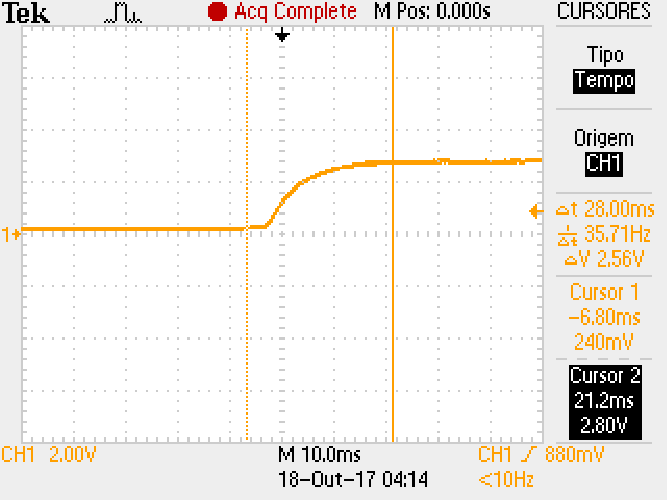
\includegraphics[width=\textwidth,height=\textheight,keepaspectratio]{figuras/TestePololu1mm.pdf}
         \caption{\centering \label{fig:TestePololu1mm}}
     \end{subfigure}

	\caption{Teste dos sensores a 1mm de distância (a) QRE1113 do Aliexpress; (b) QRE1113 da Arrow; (c) QRD1114; (d) QTR-1A}
 \end{figure}
\end{frame}


\begin{frame}
\frametitle{Teste dos sensores de refletância}
\begin{figure}[h]
     \centering
     \captionsetup{width=0.8\textwidth,font=footnotesize,textfont=bf}
     \begin{subfigure}[b]{0.3\textwidth}
 	\centering
         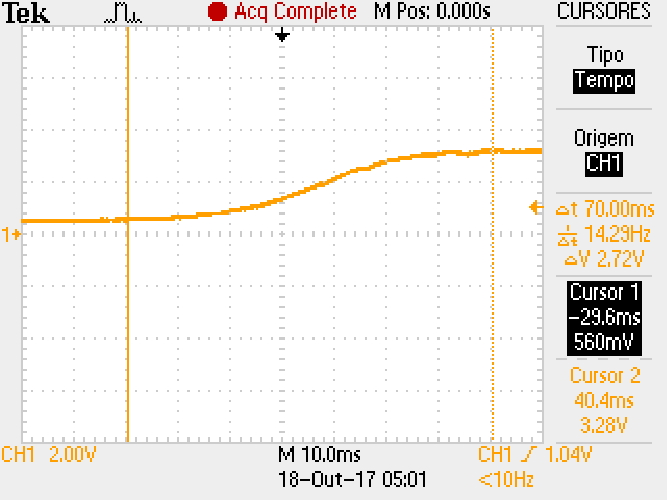
\includegraphics[width=\textwidth,height=\textheight,keepaspectratio]{figuras/TesteNew2mm.pdf}
         \caption{\centering \label{fig:TesteNew2mm}}
     \end{subfigure}
     ~
     \begin{subfigure}[b]{0.3\textwidth}
 	\centering
         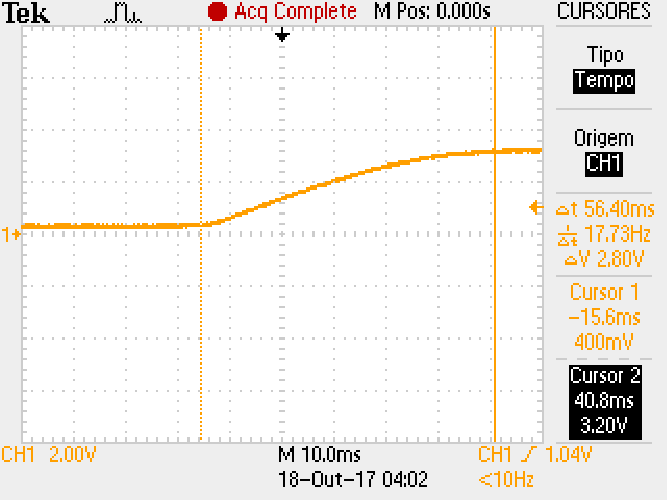
\includegraphics[width=\textwidth,height=5\textheight,keepaspectratio]{figuras/TesteOld2mm.pdf}
         \caption{\centering \label{fig:TesteOld2mm}}
     \end{subfigure}
     
     \captionsetup{width=\textwidth,font=footnotesize,textfont=bf}
     \begin{subfigure}[b]{0.3\textwidth}
 	\centering
         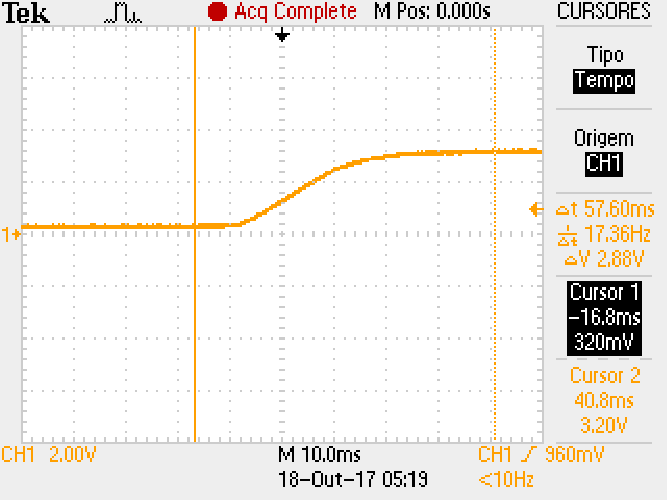
\includegraphics[width=\textwidth,height=\textheight,keepaspectratio]{figuras/TestePaulo2mm.pdf}
         \caption{\centering \label{fig:TestePaulo2mm}}
     \end{subfigure}
     ~ 
     \begin{subfigure}[b]{0.3\textwidth}
 	\centering
         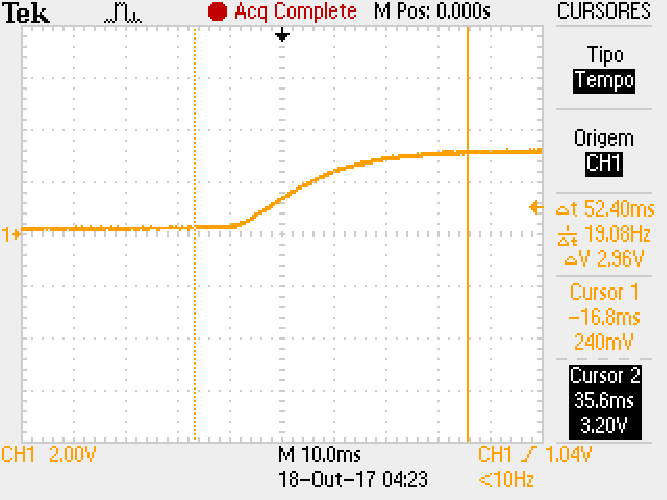
\includegraphics[width=\textwidth,height=\textheight,keepaspectratio]{figuras/TestePololu2mm.pdf}
         \caption{\centering \label{fig:TestePololu2mm}}
     \end{subfigure}

     \caption{Resposta do sensores a 2 mm de distância: (a) QRE1113 do Aliexpress; (b) QRE1113 da Arrow; (c) QRD1114; (d) QTR-1A}

 \end{figure}
\end{frame}


%%%%%%%%%%%%%%%%%%%%% EOF %%%%%%%%%%%%%%%%%%%%%%%